\documentclass[a4paper]{article}

\usepackage{array}
\usepackage{listings}
\usepackage{appendix}
\usepackage{hyperref}
\usepackage{graphicx}
\usepackage{numprint}
\usepackage{booktabs}

\usepackage{hyperref}
\hypersetup{
  colorlinks=true,
  linkcolor=blue,
  filecolor=magenta,
  urlcolor=cyan,
}
\npdecimalsign{.}
\nprounddigits{4}

\title{Algorithmic Implementation of Atmospheric Correction over Water}
\date{November 03 2019}
\author{Josh Sixsmith \& Passang Dorj}

\begin{document}
  \pagenumbering{gobble}
  \maketitle
  \newpage
  \pagenumbering{arabic}

  \section{Introduction}

    \begin{flushleft}
      This document provides a brief overview of the implementation of atmospheric correction over water surfaces. The implementation is based on information provided in \url{https://www.mssanz.org.au/modsim2017/G9/li.pdf}. \par
      The algorithm and workflow has been implemented into the \textit{wagl} codebase (\url{https://www.github.com/GeoscienceAustralia/wagl}). A key component to the algorithmic implementation is the derivation and application of a point spread function representing the atmosphere. \par
      The PSF is applied via image convolution, and depending on the resolution of the image, a kernel representing the PSF could be very large. This can present an issue for a production system when using standard image convolution. As such, two methods of convolution were implemented, and both versions will be compared and discussed.
    \end{flushleft}

  \section{Implementation details}

  \subsection{Derivation of the atmospheric PSF}

    \begin{flushleft}
      We have been supplied a build of MODTRAN (version 5.4) that has been internally modified in order in order to output the atmospheric PSF. \par
      The wagl codebase makes use of MODTRAN 6.0, and rather than fall back to using MODTRAN 5.4, it was decided to keep using MODTRAN 6.0 for the radiative transfer component, and only use MODTRAN 5.4 for retrieving the PSF. \par
      The supplied version of MODTRAN 5.4 was further modified in order to output the channel names that a calculated PSF refers to. The modification enabled a simpler workflow that relied on no assumptions about a given sensor, or for the channel order. The outputs are still appended to the TP7 file. \par
      The PSF is read and stored (along with all the outputs produced by wagl) in an HDF5 file, as well as the 2D kernel representing the PSF. \par
      The kernel is stored unnormalised; however, it is normalised during the convolution process.
    \end{flushleft}

  \subsection{Aerosol type}
    \begin{flushleft}
      The aerosol type is not enabled from the command line; instead, a simple boolean switch has been implemented that specifies that an acquisition or given a set of acquisitions is to be processed via the water atmospheric correction method instead. Internally, the workflow will then use a Maritime Navy model. This behaviour could be changed, enabling a user to specify 1 of several supported aerosol models. \par
      For a production system to be designed and implemented, a logical process needs to be defined that enables automatic processing with a given aerosol. i.e. how does one determine the aerosol model for use within the workflow process? \par
      A quick solution is simply to pre-define locations to specifically use a given aerosol model. Considering the short time frames involved, the simplest approach is to process a batch job where a user specifies what model to use for each batch of processing.
    \end{flushleft}

  \subsection{Convolution (and preperation for)}

    \begin{flushleft}
      Convolution does not work effectively if the data contains null values. To avoid a null data issue, run length (or row length) averages are calculated and used as a fill value. This is a cheap and easy method to implement and compute; however, under certain conditions may not capture the spatial variability nor the context correctly. Alternate methods, such as spatial neighbourhood averaging have not been tested, but like anything, will require thorough testing and evaluation. \par
      We did uncover an issue regarding image acquisitions that don't have a tight bounding box around the data extent, i.e.\ full rows of null data located at the top and bottom of the image. We now handle this issue by reducing the image to a tight bounding box before convolution and insert the result into the full array dimensions to preserve the original extent. \par

    \begin{figure}[h!]
      \centering
      \caption{Example of a non-tight bounding box}\label{fig:1}
      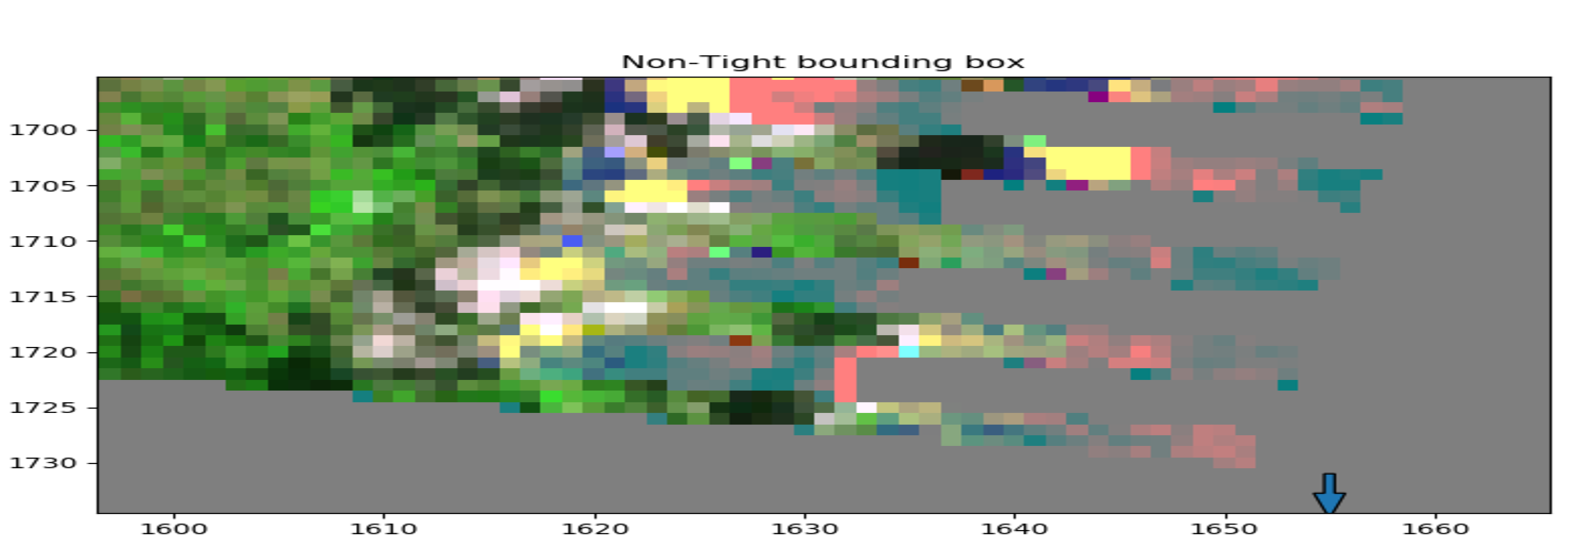
\includegraphics[scale=0.30]{non-tight-bounding-box.png}
    \end{figure}

      However, if a row of null data happens to occur between two valid rows, we call this phenomenon non-sequential and raise an Exception to stop the process. We don't anticipate coming across many acquisitions if any at all. So we felt it best to stop the process and record the acquisition id for future investigation. \par

    \begin{figure}[h!]
      \hspace*{-1.0cm}
      \centering
      \caption{Example of sequential and non-sequential data}\label{fig:2}
      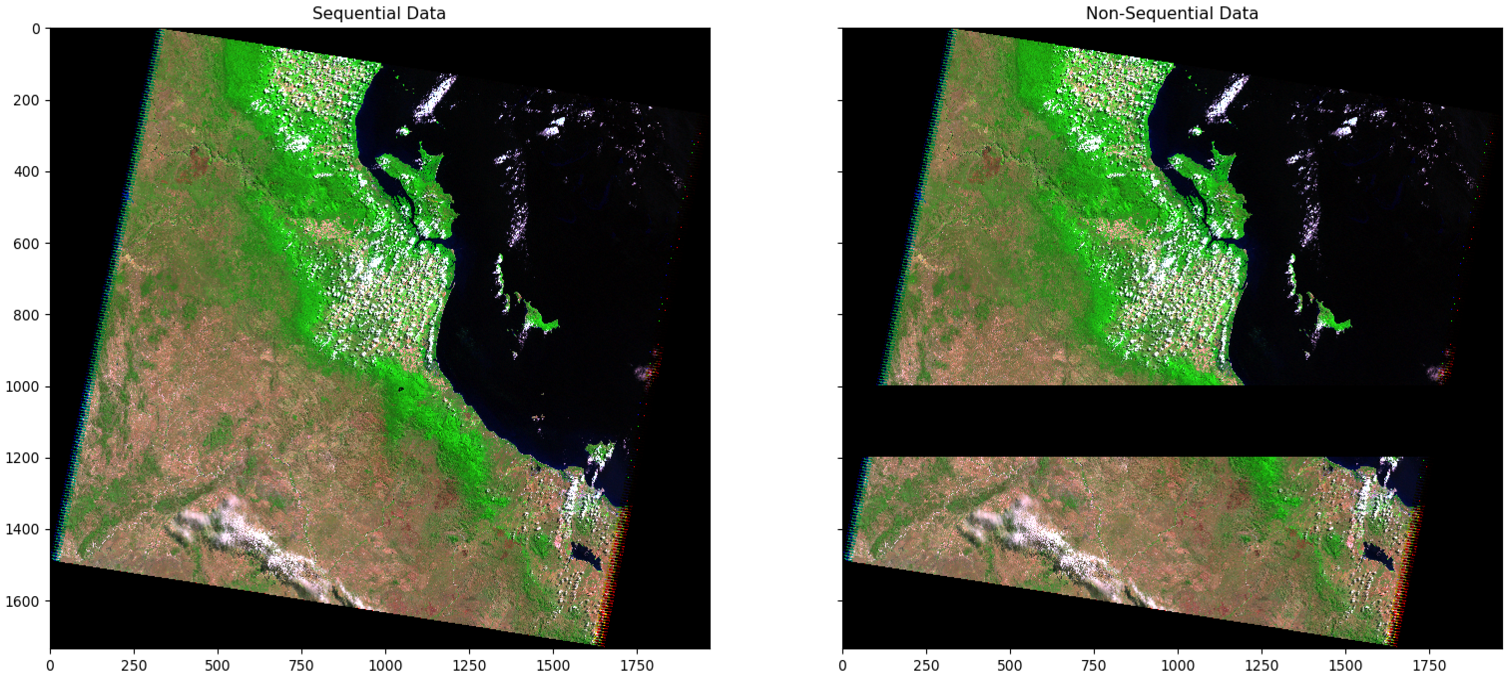
\includegraphics[scale=0.30]{sequential-non-sequential-crop.png}
    \end{figure}

    \clearpage

      Prior to convolution, both the data and the kernel are padded to an optimal size in both the x and y directions. The pad size is determined in two steps, 1. half the kernel size in each dimension + 1, 2. Find the next optimal power of 2 to enable an efficient Fourier transform. The actual padding method is \textit{symmetric} for the data and \textit{constant} for the kernel. \par
      The convolution process, depending on the dimensions of the array and the resolution, can be very time-consuming. For example, processing a (10980, 10980) image with a (141, 141) kernel took approximately 50 minutes. So for Sentinel-2, there would be an additional three images of the same dimensions to process. The current design of the workflow isn't geared towards parallelising a single function; rather, it is geared towards parallelising across acquisitions (process more acquisitions at once). \par
      As the PSF is designed to be radially symmetric, we've also enabled convolution to occur via Fourier. This has significantly reduced the computational time, at the expense of more system memory. Processing the same image example would take approximately 3 minutes via the Fourier method.
    \end{flushleft}

  \subsection{Glint correction}

    \begin{flushleft}
      While the paper that the implementations ware based of included both a sun and sky glint correction. In consultation with Team Wombats, we have only implemented sky glint correction as an appropriate source of wind speed data has not been identified, as well as the fact that more work is required to develop an appropriate method that accounts for the high spatial variability of wind speed. \par
      As for sky glint correction, a value of 1.34 for the refractive water index has been hardcoded. If desirable, the refractive water index can be added to the command line. Alternatively, wagl can be imported as a standard Python module, and the functions separately and define a value for the refractive water index as a keyword argument. \par
      We were provided with outputs from a sample dataset to use as a comparison, but we were unable to get a satisfyingly close value on a simple image difference. As such, we then turned to the sample code that was provided and found that there is an additional variable \textit{scat}. \par
\(\phantom{0}\)
      \par
      The paper used this equation: 
    \end{flushleft}

    \begin{equation} \label{eq:1}
      \rho_{g} = f_{s}\rho_{sung} + (1 - f_{skyg})\rho_{skyg}
    \end{equation}

     \begin{flushleft}
      Whereas the code used:
    \end{flushleft}

    \begin{equation} \label{eq:2}
      \rho_{g} = f_{s}\rho_{sung} + ((1 - f_{skyg})+scat)\rho_{skyg}
    \end{equation}

    \begin{flushleft}
      Equation~\ref{eq:2} yielded results that were slightly closer to the sample dataset, but still not the same. Despite the difference in results, equation~\ref{eq:2} has been implemented and is in use by the workflow.
    \end{flushleft}

  \section{Outputs}

    \subsection{Sample package}

    \begin{flushleft}
      The current output package is not a representation of the final package. Additional work is required to determine the minimum requirements that meet the need for downstream applications relying on the atmospheric correction over water product. \par
      The test output package contains:
    \end{flushleft}

      \begin{itemize}
        \item \small{Lambertian Reflectance}
        \item \small{Lambertian reflectance with atmospheric adjacency correction}
        \item \small{NBAR (using adjacency corrected lambertian as input)}
        \item \small{NBART (using adjacency corrected lambertian as input)}
        \item \small{Fmask (classification schema identifing clear, cloud, cloud shadow, water and snow pixels)}
        \item \small{FV (Direct fraction in the view direction)}
        \item \small{Azimuthal incident and exiting angles}
        \item \small{Incident and exiting angles}
        \item \small{Relative azimuth and relative slope}
        \item \small{terrain shadow (cast and self shadow)}
        \item \small{satellite azimuth and satellite view}
        \item \small{solar azimuth and solar zenith}
        \item \small{time delta of the sensor acquisition}
      \end{itemize}

    \begin{flushleft}
      The outputs will be made available via an opendatacube instance, and the database location and product name will be provided soon. At this stage, the access will be via NCI, but if desireable, some work could be done to make the data available via an EC2 \url{https://aws.amazon.com/ec2/} instance on Amazon Web Services \url{https://aws.amazon.com/} running opendatacube. \par
      While the paper mentioned not applying the point spread function to channels measuring across the SWIR domain, we decided not to include that logic here. The reasoning was mostly a consideration of timing constraints; however, if desired for the next phase of testing and validation, this work can be done. But it may also depend on defining what is required to be contained within the \textit{atmospheric correction over water} product and what processes are to be applied to each channel. \par

    \clearpage

      The following lists what channels will be output for each sensor as part of this initial implementation:
    \end{flushleft}

    \begin{itemize}
      \item \small{Landsat-5 TM Channels:}
        \begin{itemize}
          \item \footnotesize{BAND 1 (Blue)}
          \item \footnotesize{BAND 2 (Green)}
          \item \footnotesize{BAND 3 (Red)}
          \item \footnotesize{BAND 4 (NIR)}
          \item \footnotesize{BAND 5 (SWIR 1)}
          \item \footnotesize{BAND 7 (SWIR 2)}
        \end{itemize}
      \item \small{Landsat-7 ETM+ Channels:}
        \begin{itemize}
          \item \footnotesize{BAND 1 (Blue)}
          \item \footnotesize{BAND 2 (Green)}
          \item \footnotesize{BAND 3 (Red)}
          \item \footnotesize{BAND 4 (NIR)}
          \item \footnotesize{BAND 5 (SWIR 1)}
          \item \footnotesize{BAND 7 (SWIR 2)}
          \item \footnotesize{BAND 8 (Panchromatic)}
        \end{itemize}
      \item \small{Landsat-8 OLI Channels:}
        \begin{itemize}
          \item \footnotesize{BAND 1 (Coastal Aerosol)}
          \item \footnotesize{BAND 2 (Blue)}
          \item \footnotesize{BAND 3 (Green)}
          \item \footnotesize{BAND 4 (Red)}
          \item \footnotesize{BAND 5 (NIR)}
          \item \footnotesize{BAND 6 (SWIR 1)}
          \item \footnotesize{BAND 7 (SWIR 2)}
          \item \footnotesize{BAND 8 (Panchromatic)}
        \end{itemize}
      \item \small{Sentinel-2 MSI Channels:}
        \begin{itemize}
          \item \footnotesize{BAND 1 (Coastal Aerosol)}
          \item \footnotesize{BAND 2 (Blue)}
          \item \footnotesize{BAND 3 (Green)}
          \item \footnotesize{BAND 4 (Red)}
          \item \footnotesize{BAND 5 (Red Edge 1)}
          \item \footnotesize{BAND 6 (Red Edge 2)}
          \item \footnotesize{BAND 7 (Red Edge 3)}
          \item \footnotesize{BAND 8 (NIR 1)}
          \item \footnotesize{BAND 8A (NIR 2)}
          \item \footnotesize{BAND 11 (SWIR 2)}
          \item \footnotesize{BAND 12 (SWIR 3)}
        \end{itemize}
    \end{itemize}

    \section{Results}

    \subsection{Processing comparison of convolution methods}

    \begin{flushleft}
      In total, 16 acquisitions across four different sensors were used for testing, not just the algorithmic additions, but also the framework and its ability to be applied generally across different satellite acquisitions and different resolutions. The acquisitions tested are listed below:
    \end{flushleft}

      \begin{enumerate}
        \item \footnotesize{LT05\_L1TP\_093086\_20041210\_20161127\_01\_T1.tar}
        \item \footnotesize{LT05\_L1TP\_093086\_19991127\_20161216\_01\_T1.tar}
        \item \footnotesize{LT05\_L1TP\_095073\_20080915\_20161029\_01\_T1.tar}
        \item \footnotesize{LE07\_L1TP\_093086\_20081111\_20161224\_01\_T1.tar}
        \item \footnotesize{LE07\_L1TP\_093086\_20010617\_20170205\_01\_T1.tar}
        \item \footnotesize{LE07\_L1TP\_095073\_20070516\_20170103\_01\_T1.tar}
        \item \footnotesize{LC08\_L1TP\_093086\_20141020\_20170418\_01\_T1.tar}
        \item \footnotesize{LC08\_L1TP\_093086\_20151226\_20170331\_01\_T1.tar}
        \item \footnotesize{LC08\_L1TP\_095073\_20130828\_20170502\_01\_T1.tar}
        \item \footnotesize{LC08\_L1TP\_097084\_20171211\_20171223\_01\_T1.tar}
        \item \footnotesize{LC08\_L1TP\_110073\_20150624\_20170407\_01\_T1.tar}
        \item \footnotesize{LC08\_L1TP\_112083\_20151113\_20170402\_01\_T1.tar}
        \item \footnotesize{LC08\_L1TP\_115078\_20130707\_20170503\_01\_T1.tar}
        \item \footnotesize{S2A\_MSIL1C\_20190401T002101\_N0207\_R116\_T55HBU\_20190401T014505.zip}
        \item \footnotesize{S2B\_MSIL1C\_20190403T001109\_N0207\_R073\_T55HBU\_20190403T013318.zip}
        \item \footnotesize{S2A\_MSIL1C\_20190723T020451\_N0208\_R017\_T51KVA\_20190723T033407.zip}
      \end{enumerate}

    \begin{flushleft}
      The first comparison is looking at the processing efficiency and the memory overhead to get an idea of how much time is required for processing a batch of acquisitions, and the memory requirement which can limit how many acquisitions can be processed in parallel on a single node. \par
      It should be noted that the following tables are not reporting the processing time and memory usage of convolution. The reported metrics are, in fact, of the entire workflow that outputs surface reflectance.
    \end{flushleft}

    \begin{table}[ht!]
      \caption{Processing time and memory usage}\label{table:1}
      \centering
      \begin{tabular}{ccc} \midrule
        \textbf{Method} & \textbf{Walltime} & \textbf{Memory} \\ \midrule
        Standard Convolution & 07:32:18 & 64.0GB \\
        Convolution via Fourier & 00:50:30 & 55.45GB \\ \midrule
      \end{tabular}
    \end{table}

    \begin{flushleft}
      As you can see, convolution via Fourier is much more efficient both in processing time, and only slightly more efficient in memory usage. But I would like to point out that this is merely comparing the time taken and memory used for processing the test acquisitions as a single batch job. The assumption is that for the standard convolution processing, the bulk of the time would be taken up by processing the higher-resolution channels.
    \end{flushleft}

    \begin{table}[ht!]
      \caption{Per sensor processing time and memory usage (convolution via Fourier)}\label{table:2}
      \centering
      \begin{tabular}{ccc} \midrule
        \textbf{Sensor} & \textbf{Walltime} & \textbf{Memory} \\ \midrule
        TM & 00:22:22 & 1GB \\
        ETM & 00:52:19 & 7.68GB \\
        OLI & 00:43:23 & 9.02GB \\
        MSI & 00:56:10 & 4.61GB \\ \midrule
      \end{tabular}
    \end{table}

    \begin{flushleft}
      While the wall times for ETM and MSI are longer than the 50 minutes wall time reported in Table~\ref{table:1}, it should be noted that the times reported are from singular job runs. For a more realistic estimate, each job should ideally be run about half a dozen times each and an aggregate time reported. Unfortunately, with the timing constraints of this project, this will suffice. If a more accurate estimate is desired, this can be done at a more convenient time. \par
      It should also be noted that the reported memory use comes directly from the PBS job status report and not from a memory profiling tool. The reported memory use is determined by a job monitoring tool managed by NCI and executed intermittently. As such, it will only be an estimate, and if a more accurate memory profile is desired, this can be done at a more convenient time.
    \end{flushleft}

    \begin{table}[ht!]
      \caption{Per sensor processing time and memory usage per sensor (standard convolution)}\label{table:3}
      \centering
      \begin{tabular}{ccc} \midrule
        \textbf{Sensor} & \textbf{Walltime} & \textbf{Memory} \\ \midrule
        TM & 00:22:33 & 2.25GB \\
        ETM & 01:09:10 & 6.11GB \\
        OLI & 01:13:12 & 6.53GB \\
        MSI & 06:37:35 & 13.86GB \\ \midrule
      \end{tabular}
    \end{table}

    \begin{flushleft}
      From Table~\ref{table:3}, it is clear that there is a significant difference in wall time for those sensors that have higher resolution channels to process. With the MSI sensor topping the lot at just over 6.5 hours. \par
      The processing times could be reduced in various ways, such as process each band independently; however, in simply changing the method, we can reduce the time significantly. Reducing the kernel size is another, however further testing on the impact of limiting the kernel size is required.
    \end{flushleft}

    \subsection{Output comparison of convolution methods}

    \begin{flushleft}
      The following section is a simple difference comparison of the two different methods of applying convolution. The idea being that if the results come out vastly different, or simply not to an acceptable standard, then the alternate method (in this case using Fourier) will be abandoned. \par
      The image datasets that used for comparison are all \textit{atmoshperic adjacency corrected Lambertian reflectance}. If anything is wrong with this level of data output, then all datasets that use this as input are likely to be affected themselves.
    \end{flushleft}

    \begin{table}[ht!]
      \caption{LT05\_L1TP\_093086\_20041210\_20161127\_01\_T1.tar}\label{table:4}
      \centering
      \small
      \begin{tabular}{ccccc} \midrule
        \textbf{Channel name} & \textbf{Min difference} & \textbf{Max difference} & \textbf{Percent different} \\ \midrule
        BAND 1 & 0 & 0 & 0 \\
        BAND 2 & 0 & 0 & 0 \\
        BAND 3 & 0 & 0 & 0 \\
        BAND 4 & 0 & 0 & 0 \\
        BAND 5 & 0 & 0 & 0 \\
        BAND 7 & 0 & 0 & 0 \\ \midrule
      \end{tabular}
    \end{table}

    \begin{table}[ht!]
      \caption{LT05\_L1TP\_093086\_19991127\_20161216\_01\_T1.tar}\label{table:5}
      \centering
      \small
      \begin{tabular}{ccccc} \midrule
        \textbf{Channel name} & \textbf{Min difference} & \textbf{Max difference} & \textbf{Percent different} \\ \midrule
        BAND 1 & 0 & 0 & 0 \\
        BAND 2 & 0 & 0 & 0 \\
        BAND 3 & 0 & 0 & 0 \\
        BAND 4 & 0 & 0 & 0 \\
        BAND 5 & 0 & 0 & 0 \\
        BAND 7 & 0 & 0 & 0 \\ \midrule
      \end{tabular}
    \end{table}

    \begin{table}[ht!]
      \caption{LT05\_L1TP\_095073\_20080915\_20161029\_01\_T1.tar}\label{table:6}
      \centering
      \small
      \begin{tabular}{ccccc} \midrule
        \textbf{Channel name} & \textbf{Min difference} & \textbf{Max difference} & \textbf{Percent different} \\ \midrule
        BAND 1 & 0 & 0 & 0 \\
        BAND 2 & 0 & 0 & 0 \\
        BAND 3 & 0 & 0 & 0 \\
        BAND 4 & 0 & 0 & 0 \\
        BAND 5 & 0 & 0 & 0 \\
        BAND 7 & 0 & 0 & 0 \\ \midrule
      \end{tabular}
    \end{table}

  \clearpage

    \begin{table}[ht!]
      \caption{LE07\_L1TP\_093086\_20081111\_20161224\_01\_T1.tar}\label{table:7}
      \centering
      \small
      \begin{tabular}{ccccc} \midrule
        \textbf{Channel name} & \textbf{Min difference} & \textbf{Max difference} & \textbf{Percent different} \\ \midrule
        BAND 1 & 0 & 0 & 0 \\
        BAND 2 & 0 & 0 & 0 \\
        BAND 3 & 0 & 0 & 0 \\
        BAND 4 & 0 & 0 & 0 \\
        BAND 5 & 0 & 0 & 0 \\
        BAND 7 & 0 & 0 & 0 \\
        BAND 8 & 0 & 0 & 0 \\ \midrule
      \end{tabular}
    \end{table}

    \begin{table}[ht!]
      \caption{LE07\_L1TP\_093086\_20010617\_20170205\_01\_T1.tar}\label{table:8}
      \centering
      \small
      \begin{tabular}{ccccc} \midrule
        \textbf{Channel name} & \textbf{Min difference} & \textbf{Max difference} & \textbf{Percent different} \\ \midrule
        BAND 1 & 0 & 0 & 0 \\
        BAND 2 & 0 & 0 & 0 \\
        BAND 3 & 0 & 0 & 0 \\
        BAND 4 & 0 & 0 & 0 \\
        BAND 5 & 0 & 0 & 0 \\
        BAND 7 & 0 & 0 & 0 \\
        BAND 8 & 0 & 0 & 0 \\ \midrule
      \end{tabular}
    \end{table}

    \begin{table}[ht!]
      \caption{LE07\_L1TP\_095073\_20070516\_20170103\_01\_T1.tar}\label{table:9}
      \centering
      \small
      \begin{tabular}{ccccc} \midrule
        \textbf{Channel name} & \textbf{Min difference} & \textbf{Max difference} & \textbf{Percent different} \\ \midrule
        BAND 1 & 0 & 0 & 0 \\
        BAND 2 & 0 & 0 & 0 \\
        BAND 3 & 0 & 0 & 0 \\
        BAND 4 & 0 & 0 & 0 \\
        BAND 5 & 0 & 0 & 0 \\
        BAND 7 & 0 & 0 & 0 \\
        BAND 8 & 0 & 0 & 0 \\ \midrule
      \end{tabular}
    \end{table}

    \begin{table}[ht!]
      \caption{LC08\_L1TP\_093086\_20141020\_20170418\_01\_T1.tar}\label{table:10}
      \centering
      \small
      \begin{tabular}{ccccc} \midrule
        \textbf{Channel name} & \textbf{Min difference} & \textbf{Max difference} & \textbf{Percent different} \\ \midrule
        BAND 1 & 0 & 0 & 0 \\
        BAND 2 & 0 & 0 & 0 \\
        BAND 3 & 0 & 0 & 0 \\
        BAND 4 & 0 & 0 & 0 \\
        BAND 5 & 0 & 0 & 0 \\
        BAND 7 & 0 & 0 & 0 \\
        BAND 6 & 0 & 0 & 0 \\
        BAND 8 & 0 & 0 & 0 \\ \midrule
      \end{tabular}
    \end{table}

  \clearpage

    \begin{table}[ht!]
      \caption{LC08\_L1TP\_093086\_20151226\_20170331\_01\_T1.tar}\label{table:11}
      \centering
      \small
      \begin{tabular}{ccccc} \midrule
        \textbf{Channel name} & \textbf{Min difference} & \textbf{Max difference} & \textbf{Percent different} \\ \midrule
        BAND 1 & 0 & 0 & 0 \\
        BAND 2 & 0 & 0 & 0 \\
        BAND 3 & 0 & 0 & 0 \\
        BAND 4 & 0 & 0 & 0 \\
        BAND 5 & 0 & 0 & 0 \\
        BAND 6 & 0 & 0 & 0 \\
        BAND 7 & 0 & 0 & 0 \\
        BAND 8 & 0 & 0 & 0 \\ \midrule
      \end{tabular}
    \end{table}

    \begin{table}[ht!]
      \caption{LC08\_L1TP\_095073\_20130828\_20170502\_01\_T1.tar}\label{table:12}
      \centering
      \small
      \begin{tabular}{ccccc} \midrule
        \textbf{Channel name} & \textbf{Min difference} & \textbf{Max difference} & \textbf{Percent different} \\ \midrule
        BAND 1 & 0 & 0 & 0 \\
        BAND 2 & 0 & 0 & 0 \\
        BAND 3 & 0 & 0 & 0 \\
        BAND 4 & 0 & 0 & 0 \\
        BAND 5 & 0 & 0 & 0 \\
        BAND 6 & 0 & 0 & 0 \\
        BAND 7 & 0 & 0 & 0 \\
        BAND 8 & 0 & 0 & 0 \\ \midrule
      \end{tabular}
    \end{table}

    \begin{table}[ht!]
      \caption{LC08\_L1TP\_097084\_20171211\_20171223\_01\_T1.tar}\label{table:13}
      \centering
      \small
      \begin{tabular}{ccccc} \midrule
        \textbf{Channel name} & \textbf{Min difference} & \textbf{Max difference} & \textbf{Percent different} \\ \midrule
        BAND 1 & 0 & 0 & 0 \\
        BAND 2 & 0 & 0 & 0 \\
        BAND 3 & 0 & 0 & 0 \\
        BAND 4 & 0 & 0 & 0 \\
        BAND 5 & 0 & 0 & 0 \\
        BAND 6 & 0 & 0 & 0 \\
        BAND 7 & 0 & 0 & 0 \\
        BAND 8 & 0 & 0 & 0 \\ \midrule
      \end{tabular}
    \end{table}

  \clearpage

    \begin{table}[ht!]
      \caption{LC08\_L1TP\_110073\_20150624\_20170407\_01\_T1.tar}\label{table:14}
      \centering
      \small
      \begin{tabular}{ccccc} \midrule
        \textbf{Channel name} & \textbf{Min difference} & \textbf{Max difference} & \textbf{Percent different} \\ \midrule
        BAND 1 & 0 & 0 & 0 \\
        BAND 2 & 0 & 0 & 0 \\
        BAND 3 & 0 & 0 & 0 \\
        BAND 4 & 0 & 0 & 0 \\
        BAND 5 & 0 & 0 & 0 \\
        BAND 6 & 0 & 0 & 0 \\
        BAND 7 & 0 & 0 & 0 \\
        BAND 8 & 0 & 0 & 0 \\ \midrule
      \end{tabular}
    \end{table}

    \begin{table}[ht!]
      \caption{LC08\_L1TP\_112083\_20151113\_20170402\_01\_T1.tar}\label{table:15}
      \centering
      \small
      \begin{tabular}{ccccc} \midrule
        \textbf{Channel name} & \textbf{Min difference} & \textbf{Max difference} & \textbf{Percent different} \\ \midrule
        BAND 1 & 0 & 0 & 0 \\
        BAND 2 & 0 & 0 & 0 \\
        BAND 3 & 0 & 0 & 0 \\
        BAND 4 & 0 & 0 & 0 \\
        BAND 5 & 0 & 0 & 0 \\
        BAND 6 & 0 & 0 & 0 \\
        BAND 7 & 0 & 0 & 0 \\
        BAND 8 & 0 & 0 & 0 \\ \midrule
      \end{tabular}
    \end{table}

    \begin{table}[ht!]
      \caption{LC08\_L1TP\_115078\_20130707\_20170503\_01\_T1.tar}\label{table:16}
      \centering
      \small
      \begin{tabular}{ccccc} \midrule
        \textbf{Channel name} & \textbf{Min difference} & \textbf{Max difference} & \textbf{Percent different} \\ \midrule
        BAND 1 & 0 & 0 & 0 \\
        BAND 2 & 0 & 0 & 0 \\
        BAND 3 & 0 & 0 & 0 \\
        BAND 4 & 0 & 0 & 0 \\
        BAND 5 & 0 & 0 & 0 \\
        BAND 6 & 0 & 0 & 0 \\
        BAND 7 & 0 & 0 & 0 \\
        BAND 8 & 0 & 0 & 0 \\ \midrule
      \end{tabular}
    \end{table}

  \clearpage

    \begin{table}[ht!]
      \caption{\footnotesize{S2A\_MSIL1C\_20190401T002101\_N0207\_R116\_T55HBU\_20190401T014505.zip}}\label{table:17}
      \centering
      \small
      \begin{tabular}{|c|n{2}{4}|n{2}{4}|n{2}{4}|n{2}{4}|} \hline
        \textbf{Channel name} & \textbf{Min difference} & \textbf{Max difference} & \textbf{Percent different} \\ \midrule
        BAND 1 & 0 & 0 & 0 \\
        BAND 2 & -1.862645149230957e-09 & 0 & 8.294597562715453e-07 \\
        BAND 3 & 0 & 0 & 0 \\
        BAND 4 & 0 & 0 & 0 \\
        BAND 5 & 0 & 0 & 0 \\
        BAND 6 & 0 & 0 & 0 \\
        BAND 7 & 0 & 0 & 0 \\
        BAND 8 & 0 & 0 & 0 \\
        BAND 8A & 0 & 0 & 0 \\
        BAND 11 & 0 & 0 & 0 \\
        BAND 12 & 0 & 0 & 0 \\ \midrule
      \end{tabular}
    \end{table}

    \begin{table}[ht!]
      \caption{\footnotesize{S2B\_MSIL1C\_20190403T001109\_N0207\_R073\_T55HBU\_20190403T013318.zip}}\label{table:18}
      \centering
      \small
      \begin{tabular}{ccccc} \midrule
        \textbf{Channel name} & \textbf{Min difference} & \textbf{Max difference} & \textbf{Percent different} \\ \midrule
        BAND 1 & 0 & 0 & 0 \\
        BAND 2 & 0 & 0 & 0 \\
        BAND 3 & 0 & 0 & 0 \\
        BAND 4 & 0 & 0 & 0 \\
        BAND 5 & 0 & 0 & 0 \\
        BAND 6 & 0 & 0 & 0 \\
        BAND 7 & 0 & 0 & 0 \\
        BAND 8 & 0 & 0 & 0 \\
        BAND 8A & 0 & 0 & 0 \\
        BAND 11 & 0 & 0 & 0 \\
        BAND 12 & 0 & 0 & 0 \\ \midrule
      \end{tabular}
    \end{table}

    \begin{table}[ht!]
      \caption{\footnotesize{S2A\_MSIL1C\_20190723T020451\_N0208\_R017\_T51KVA\_20190723T033407.zip}}\label{table:19}
      \centering
      \small
      \begin{tabular}{cn{2}{4}n{2}{4}n{2}{4}n{2}{4}} \midrule
        \textbf{Channel name} & \textbf{Min difference} & \textbf{Max difference} & \textbf{Percent different} \\ \midrule
        BAND 1 & 0 & 0 & 0 \\
        BAND 2 & 0 & 3.725290298461914e-09 & 8.294597562715453e-07 \\
        BAND 3 & 0 & 0 & 0 \\
        BAND 4 & 0 & 0 & 0 \\
        BAND 5 & 0 & 0 & 0 \\
        BAND 6 & 0 & 0 & 0 \\
        BAND 7 & 0 & 0 & 0 \\
        BAND 8 & 0 & 0 & 0 \\
        BAND 8A & 0 & 0 & 0 \\
        BAND 11 & 0 & 0 & 0 \\
        BAND 12 & 0 & 0 & 0 \\ \midrule
      \end{tabular}
    \end{table}

  \clearpage

    \begin{flushleft}
      Of all the channels from each Satellite/Sensor combination, only two bands returned a difference in the comparison of atmospheric adjacency corrected Lambertian reflectance using two different methods, \textit{standard convolution} and \textit{convolution via fourier}. The difference itself is minimal, as is the tally of pixels that are different. \par
      I would put these differences down to standard floating-point calculations, and if a 10000 scale factor is applied, the values will truncate to zero.
    \end{flushleft}

  \section{Recommendations}

    \begin{flushleft}
      From the difference comparisons on the sample datasets, it is clear that we can achieve the same or otherwise a very very similar result to standard convolution when using convolution via Fourier. \par
      The metrics gathered from each of the batch processing jobs indicate the advantage in using convolution via Fourier over standard convolution. Considering the size of the kernels could be quite large, we need to be considerate of the time it takes to process numerous datasets in an efficient manner. We can get a massive saving on CPU time, thus reducing the expenditure of KSU's. The additional memory required is not that significant, and in some cases, less. \par
      Kicking off a test job is fairly trivial, so much so that other users could do this themselves if they have additional test areas of interest.
    \end{flushleft}

  \section{Next steps}

    \begin{flushleft}
      Sample data can now be produced on a large scale, with different configurations. To progress the development of a standard packaged product, additional validation and testing are required. I would highly recommend that the previous validation exercise undertaken with CSIRO be re-visited and re-run against data produced by the \textit{wagl} codebase. This work should involve the Calibration/Validation team, who would be expected to document the procedure and enable the work to be more easily re-evaluated when required, as well as to collate and manage any ground truth data. \par
      For the product to be finalised for a production environment, work is needed to determine the required level of processing for the majority of downstream applications to take advantage of an Analysis Ready Data concept. \par

      Requirements such as:
    \end{flushleft}

    \begin{itemize}
      \item \footnotesize{\textit{what datatypes?}}
      \item \footnotesize{\textit{Is float32 required for sky glint corrected data in order to allow accurate sun glint correction?}}
      \item \footnotesize{\textit{Does the image need to be subsetted by half the kernel size to avoid image edge effects}}
      \item \footnotesize{\textit{Does the kernel need to be capped at a pre-determined x/y size?}}
      \item \footnotesize{\textit{Different image padding method}}
      \item \footnotesize{\textit{different method to replace null values?}}
    \end{itemize}

\end{document}
